\documentclass[10pt,conference]{IEEEtran}
\usepackage[utf8]{inputenc}
\usepackage[T1]{fontenc}
\usepackage{amsmath,amssymb,graphicx,booktabs,multirow,makecell,array}
\usepackage{siunitx,threeparttable,xcolor,microtype,enumitem,url}
\usepackage[hidelinks]{hyperref}
\hypersetup{pdfauthor={},pdfcreator={}}

\newcommand{\astH}{AST+Header}
\newcommand{\astN}{AST No-Header}
\newcommand{\lineH}{Line+Header}
\newcommand{\lineN}{Line No-Header}
\newcommand{\castname}{cAST}

\begin{document}

\title{An Empirical Evaluation of Source Code Chunking and Context Headers for Requirement Evidence Retrieval}

\author{\IEEEauthorblockN{Anonymous Authors}}

\maketitle

\begin{abstract}
Locating source code that evidences a technical requirement is a common need in software analysis. 
Syntax-aware chunking is motivated by its preservation of code structure, yet chunk boundaries are confounded with the context metadata prepended to each chunk. 
In this Research Preview, we cross two chunking strategies, abstract syntax tree (AST)-first chunking with line fallback and 50-line windows, with and without a hierarchical context header. 
We evaluate them on 25 job descriptions, whose required skills serve as requirements, and 40 public repositories (798 chunks), using BM25, dense retrieval, and cross-encoder reranking against 603 human-labeled pairs. 
After reranking, headers improved NDCG@10 for AST chunks from 0.345 to 0.457 (Holm-adjusted $p = 0.0031$), and without headers, line windows outperformed AST chunks (0.470 vs. 0.345, $p_{\mathrm{Holm}} = 0.0001$). 
We found no evidence that AST chunks with headers differ from line windows without headers ($\Delta = -0.014$, $p_{\mathrm{Holm}} = 0.85$). 
Line windows with headers scored highest (0.499), not significantly above AST with headers in an exploratory comparison. 
About 36\% of AST-arm chunks fell back to line windows, and 25 queries limit power for small differences. 
We outline a plan to isolate header components, reduce fallbacks, and validate retrieved evidence with human judgments.
\end{abstract}

\begin{IEEEkeywords}
Source code retrieval, code chunking, abstract syntax trees, context headers, requirements traceability, empirical software engineering
\end{IEEEkeywords}

\section{Introduction}
\label{sec:intro}

Locating code that provides evidence for a written requirement is a recurring need in software analysis, for example when checking whether a repository supports the requirements of a task. 
Tracing requirements to code has a long history in software engineering~\cite{antoniol2002traceability,gao2024triad,kuang2023analyzing}. 
We study a traceability-style variant: given a technical requirement phrased in natural language, here a skill required by a job description (JD), retrieve the code chunks that evidence it.

Chunking via abstract syntax trees (ASTs) is motivated by the observation that line-based splitting can break semantic structures~\cite{zhang2025cast}. 
Recent controlled evidence in code completion, however, finds that structure-aware chunking does not outperform a simple sliding window~\cite{wu2026chunking}, and another study of code-RAG design choices reports that line-based chunking matches syntax-aware splitting across context budgets~\cite{galimzyanov2025practical}. 
Whether this holds when the goal is to retrieve evidence for a requirement is unclear to us. 
Moreover, real-world source files can contain constructs, such as declarative configurations, UI templates, and type declarations, that standard method-level AST extraction does not cover, and chunk boundaries are often confounded with the metadata (e.g., file path, class name) prepended to chunks. 
To the best of our knowledge, no prior study crosses chunking strategy with context headers for requirement-to-code evidence retrieval with human relevance labels.

In this Research Preview, we investigate how chunk boundary formulation and contextual metadata interact to determine retrieval effectiveness. 
We formulate four research questions:
\begin{itemize}[leftmargin=*,itemsep=1pt,topsep=1pt]
    \item \textbf{RQ1 (Preliminary):} Does prepending a hierarchical context header improve the retrieval of requirement evidence from source code chunks?
    \item \textbf{RQ2 (Preliminary):} Does AST-first chunking outperform line-window chunking when both conditions use, or both omit, context headers?
    \item \textbf{RQ3 (Planned):} Which context header components drive retrieval improvements, and how do chunking trade-offs generalize across programming paradigms?
    \item \textbf{RQ4 (Planned):} Does retrieved code evidence improve human evaluators' accuracy and confidence in downstream requirement verification?
\end{itemize}

To address RQ1 and RQ2, we run a controlled $2 \times 2$ factorial experiment on 25 public JDs and 40 open-source repositories (20 Java Spring Boot, 20 React/TypeScript; 798 chunks) at three retrieval tiers (BM25, dense BGE-M3, and cross-encoder reranking). 
Preliminarily, headers improve reranking of AST chunks ($\Delta = +0.112$, $p_{\mathrm{Holm}} = 0.0031$); without headers, line windows outperform AST chunks ($\Delta = -0.126$, $p_{\mathrm{Holm}} = 0.0001$); and we find no evidence that AST chunks with headers differ from line windows without headers ($\Delta = -0.014$, $p_{\mathrm{Holm}} = 0.85$).

We make four contributions:
\begin{enumerate}[leftmargin=*,itemsep=1pt,topsep=1pt]
    \item A factorial design that crosses chunking strategy with context headers for requirement-to-code evidence retrieval over multi-file repositories.
    \item Preliminary findings: headers improve reranking of AST chunks, headerless line windows outperform AST chunks, and we find no evidence that AST chunks with headers differ from headerless line windows; an audit shows that 35.7\% of AST-arm chunks are line-window fallbacks.
    \item A replication package with 603 human-labeled JD-chunk pairs (weighted kappa 0.78 overall, 0.88 on the initial gold subset, and 0.68 on the pooled items) and retrieval runs.
    \item A research plan to test why headers help and whether retrieved evidence supports human verification.
\end{enumerate}
The study relates to SANER topics on software analysis, mining software repositories, and program comprehension.

\section{Related Work}
\label{sec:related_work}

We organize related work into four areas: code chunking for retrieval-augmented generation, dense code retrieval with reranking, context enrichment, and requirements traceability with skill mining.

\subsection{Code Chunking for Retrieval-Augmented Generation}
Line-based chunking can split functions or merge unrelated code~\cite{zhang2025cast}. 
\castname~\cite{zhang2025cast} addresses this by recursively splitting large AST nodes and merging sibling nodes under size limits, and reports gains on RepoEval retrieval and SWE-bench generation. 
Later controlled evidence is less favorable to structure: Wu et al.~\cite{wu2026chunking} compared four chunking strategies (function, declaration, sliding window, and \castname) for retrieval-augmented code completion and found that structure-aware strategies did not outperform a sliding window, with function-level chunking performing worst; Galimzyanov et al.~\cite{galimzyanov2025practical} likewise report that line-based chunking matches syntax-aware splitting across context budgets. 
These studies target code completion and related tasks. 
We study human-labeled requirement-to-code evidence retrieval and also cross chunking with context headers.

\subsection{Dense Code Retrieval and Reranking}
Neural code search maps natural-language queries and code into a shared vector space~\cite{feng2020codebert,guo2022unixcoder,husain2019codesearchnet}, and multilingual embedders such as BGE-M3~\cite{chen2024bgem3} encode queries and chunks independently. 
Because a bi-encoder compresses a chunk into one vector, pipelines often add a cross-encoder that re-ranks the top candidates~\cite{hu2023revisiting,costv2024apsec}: TOSS~\cite{hu2023revisiting} combines IR-based and bi-encoder recall with cross-encoder reranking, and CoSTV~\cite{costv2024apsec} uses a two-stage design to reduce search time while retaining accuracy. 
We use the same recall-then-rerank structure and ask how chunk shape and headers interact with the reranker.

\subsection{Context Enrichment}
Isolated chunks can lack the surrounding class and package context. 
RepoCoder~\cite{zhang2023repocoder} retrieves repository context iteratively to improve completion, and RepoBench~\cite{liu2024repobench} and CrossCodeEval~\cite{ding2023crosscodeeval} benchmark repository-level completion that needs cross-file context. 
These works enrich the prompt with retrieved context. 
We ask a narrower question: does a short hierarchical header prepended to each chunk change retrieval, and does it do so equally for AST chunks and line windows?

\subsection{Requirements Traceability and Skill Mining}
Tracing natural-language requirements to code is a long-standing problem~\cite{antoniol2002traceability}; recent work addresses the abstraction gap between artifacts~\cite{gao2024triad} and the evolution of trace links~\cite{kuang2023analyzing}. 
Separately, repository mining has been used to estimate developer expertise; for example, Montandon et al.~\cite{montandon2019identifying} predicted expertise in libraries and frameworks from GitHub activity using machine-learning classifiers with survey-based ground truth. 
We take the traceability view: a required skill is treated as a requirement, and we ask which code chunks evidence it. 
We do not assess individual developers.

\section{Approach and Study Design}
\label{sec:approach}

To separate chunk boundaries from context metadata, we use a $2 \times 2$ factorial design evaluated at three retrieval tiers, with an analysis plan frozen before the evaluation runs.

\subsection{Corpus and Query Curation}
Our corpus comprises 40 open-source GitHub repositories (20 Java Spring Boot, 20 React/TypeScript), encompassing 189 source files. 
Repository licenses include 19 MIT (47.5\%), 16 Public GitHub default copyright (40.0\%), 4 Apache-2.0 (10.0\%), and 1 GNU AGPL-3.0 (2.5\%). 
Requirements are extracted from 25 public job descriptions (15 Java backend, 10 React/TypeScript frontend) with a frozen prompt run on \texttt{gemini-1.5-flash} (recorded in \texttt{queries\_frozen.json}); each query lists the mandatory skills.

\subsection{Factorial Conditions and Retrieval Pipeline}
We evaluate two orthogonal factors:
\begin{enumerate}[leftmargin=*,itemsep=1pt,topsep=1pt]
    \item \textbf{Chunking Strategy:}
    \textit{Line-window chunking} slices source code into 50-LOC windows with a 10-LOC overlap (step 40 LOC), representing the standard language-agnostic baseline. 
    \textit{AST-first chunking with line fallback (AST arm)} uses Tree-sitter to parse source files into concrete syntax trees, extracting discrete functional boundaries (\texttt{method\_declaration}, \texttt{constructor\_declaration}, \texttt{arrow\_function}, and function expressions). 
    When a file has no extractable function (e.g., top-level JSX, styled-components, type declarations, or configuration objects), the parser falls back to 50-LOC windows so that such files remain searchable. 
    In total, our corpus yields 434 line chunks and 364 AST-arm chunks (234 pure AST method extractions, 130 line-window fallback chunks).
    \item \textbf{Context Header Condition:}
    In the \textit{Without Header} condition, chunks contain solely the raw code text. 
    In the \textit{With Header} condition, chunks are prepended with a standardized hierarchical context prefix: \texttt{// File: <path> \textbackslash n // Class: <name> \textbackslash n // Method: <name> \textbackslash n // Lines: <start>-<end>}.
\end{enumerate}

Each of the four resulting factorial configurations is evaluated across three retrieval tiers:
\textit{Tier 1 (Lexical):} Okapi BM25.
\textit{Tier 2 (Dense Bi-Encoder):} BAAI/bge-m3~\cite{chen2024bgem3} (1024-dimensional embeddings, cosine similarity).
\textit{Tier 3 (Two-Stage Cross-Encoder Reranking):} BAAI/bge-reranker-base~\cite{xiao2023cpack}, which jointly encodes the query and chunk and rescores the top-20 candidates from Tier 2.

\subsection{Human Annotation and Pooling Protocol}
For the 353 items added by pooling, annotators saw only the JD requirement, the file path, the line range, and the code; chunking strategy, header condition, retrieval tier, and scores were hidden. 
The 250 gold items were labeled earlier, and those annotators may have seen header information; we did not run a header-bias check. 
Two software engineering annotators labeled each pair independently on a 0--2 relevance scale (0: irrelevant; 1: partially relevant; 2: relevant), and a Lead Adjudicator resolved 122 disagreements using structured templates. 
Quadratic-weighted Cohen's kappa is 0.78 on all 603 pairs (79.8\% exact agreement), 0.88 on the 250 gold items, and 0.68 on the 353 pooled items: substantial agreement overall on the Landis-Koch scale~\cite{landis1977measurement}, but the target of 0.80 set in the annotation guidelines was met only on the gold subset.

\subsection{Evaluation Metrics and Statistical Testing}
The primary evaluation metric is Normalized Discounted Cumulative Gain at rank 10 ($\text{NDCG@10}$), computed with linear relevance gain ($rel_i / \log_2(i+1)$). 
Unjudged items are counted as relevance 0. 
Secondary metrics are $\text{NDCG@1}$ and $\text{MRR@10}$ (Table~\ref{tab:main}).

The confirmatory family specified in the frozen analysis plan comprises four paired comparisons over the 25 JDs at the reranking tier:
\begin{itemize}[leftmargin=*,itemsep=1pt,topsep=1pt]
    \item \textbf{Comp 1:} \astH\ vs. \lineN.
    \item \textbf{Comp 2:} \astN\ vs. \lineN.
    \item \textbf{Comp 3:} \astH\ vs. \astN.
    \item \textbf{Comp 4:} \lineH\ vs. \lineN.
\end{itemize}
Hypotheses are tested via two-sided Wilcoxon signed-rank tests~\cite{wilcoxon1945individual} with Holm correction~\cite{holm1979simple} ($\alpha = 0.05$). 
We report paired effect sizes $\Delta = \mathrm{mean}(A) - \mathrm{mean}(B)$ alongside 95\% bootstrap confidence intervals (10,000 resamples across queries). 
In addition, we report one exploratory contrast outside the confirmatory family: \textbf{Comp 5} (\astH\ vs. \lineH).

\section{Preliminary Results}
\label{sec:results}

\subsection{Overall Retrieval Effectiveness}
Table~\ref{tab:main} summarizes retrieval performance across all configurations and tiers. 
At the two-stage reranking tier, \lineH\ achieves the highest aggregate effectiveness ($\text{NDCG@10} = 0.499$, 95\% CI $[0.450, 0.543]$), alongside the strongest Top-1 accuracy ($\text{NDCG@1} = 0.800$) and reciprocal rank ($\text{MRR@10} = 0.980$). 
\astH\ achieves $\text{NDCG@10} = 0.457$ ($[0.405, 0.509]$), followed by \lineN\ ($0.470$, $[0.414, 0.524]$) and \astN\ ($0.345$, $[0.299, 0.390]$).

Lexical BM25 scores low in all conditions (NDCG@10 between $0.104$ and $0.187$ across the four BM25 configurations in the package; Table~\ref{tab:main} lists the two with headers). 
Because BM25 was not used for pooling, most of its top-10 items are unjudged (Judged@10 $13.6\%$--$30.4\%$ across the four configurations) and count as zero; we therefore also report bpref, which ignores unjudged items~\cite{buckley2004bpref}. 
BM25 remains lowest (bpref $0.152$--$0.241$ across configurations) but the gap to the dense ($0.278$--$0.350$) and reranking tiers ($0.285$--$0.356$) is smaller than NDCG@10 suggests. 
BM25 still serves only as a reference, not as an unpenalized baseline. 
With headers, dense retrieval improves NDCG@10 over BM25 by $0.238$ to $0.322$, and reranking adds a further $0.048$ to $0.049$. 
Notably, context headers benefit AST chunks already at the dense bi-encoder tier ($\Delta = +0.088$, rising from $0.320$ to $0.408$) as well as during reranking ($\Delta = +0.112$, reaching $0.457$), confirming that headers serve as essential anchors during initial candidate retrieval. 
For the dense and reranking systems, Judged@3 is 100\% and Judged@10 is 53.6\% to 59.2\%.

\begin{table}[t]
\caption{Retrieval effectiveness ($N=25$ JDs). Rerank tier first; Dense and BM25 are reference tiers.}
\label{tab:main}
\centering\footnotesize
\setlength{\tabcolsep}{3pt}
\begin{threeparttable}
\begin{tabular}{@{}llcccc@{}}
\toprule
Chunk & Header & NDCG@10 [95\% CI] & NDCG@1 & MRR@10 & J@10\tnote{a} \\
\midrule
Line & Yes & \textbf{0.499} [0.450, 0.543] & \textbf{0.800} & \textbf{0.980} & 0.552 \\
Line & No  & \textit{0.470} [0.414, 0.524] & \textit{0.740} & 0.933 & 0.564 \\
AST  & Yes & 0.457 [0.405, 0.509] & 0.720 & \textit{0.940} & 0.564 \\
AST  & No  & 0.345 [0.299, 0.390] & 0.460 & 0.846 & 0.536 \\
\midrule
\multicolumn{6}{l}{\textit{Reference Tiers (Line+Header / AST+Header)}} \\
Dense & Yes (Line) & 0.450 [0.398, 0.502] & 0.580 & 0.913 & 0.572 \\
Dense & Yes (AST)  & 0.408 [0.346, 0.463] & 0.660 & 0.900 & 0.544 \\
BM25$^{\dagger}$ & Yes (Line) & 0.129 [0.094, 0.165] & 0.140 & 0.405 & 0.180 \\
BM25$^{\dagger}$ & Yes (AST)  & 0.170 [0.122, 0.221] & 0.080 & 0.395 & 0.244 \\
\bottomrule
\end{tabular}
\begin{tablenotes}\footnotesize
\item[] Bold: best; italic: second best within the reranking tier.
\item[a] Judged@10: share of top-10 items with a human label (unjudged count as 0).
\item[$\dagger$] BM25 was not used for pooling; scores are not an unpenalized baseline.
\end{tablenotes}
\end{threeparttable}
\end{table}


\subsection{Hypothesis Testing and Confirmatory Analyses}
Table~\ref{tab:statistical_hypothesis_tests} presents the statistical test results for the confirmatory family and the exploratory contrast.

\begin{figure}[t]
\centering
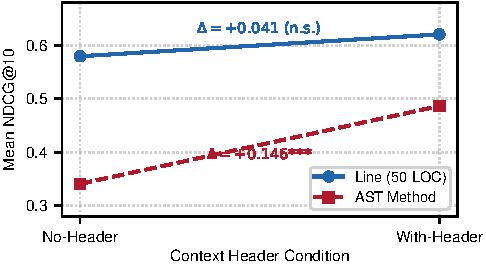
\includegraphics[width=0.88\columnwidth]{figs/fig1.pdf}
\caption{Interaction plot demonstrating differential context header sensitivity between line-window chunking and AST-first chunking at the reranking tier ($N=25$ JDs).}
\label{fig:interaction_plot}
\end{figure}

\begin{table}[t]
\caption{Hypothesis tests for the confirmatory family and the exploratory contrast (NDCG@10, rerank tier).}
\label{tab:statistical_hypothesis_tests}
\centering\footnotesize
\resizebox{\columnwidth}{!}{%
\begin{tabular}{@{}llccc@{}}
\toprule
ID & Contrast ($A - B$) & $\Delta$ [95\% CI] & W/L/T & $p_{\mathrm{Holm}}$ \\
\midrule
\multicolumn{5}{@{}l}{\emph{Confirmatory family (step-down Holm, $\alpha = 0.05$)}} \\
Comp 1 & \astH\ vs. \lineN & $-0.014$ [$-0.088$, $+0.058$] & 12/13/0 & 0.8532 \\
Comp 2 & \astN\ vs. \lineN & $-0.126$ [$-0.180$, $-0.076$] & 5/20/0  & $<0.001^{***}$ \\
Comp 3 & \astH\ vs. \astN  & $+0.112$ [$+0.056$, $+0.166$] & 19/6/0  & 0.0031$^{**}$ \\
Comp 4 & \lineH\ vs. \lineN & $+0.029$ [$-0.017$, $+0.078$] & 15/10/0 & 0.7332 \\
\midrule
\multicolumn{5}{@{}l}{\emph{Exploratory (outside the Holm family)}} \\
Comp 5 & \astH\ vs. \lineH & $-0.043$ [$-0.106$, $+0.021$] & 6/18/1  & 0.1355$^{\dagger}$ \\
\bottomrule
\end{tabular}%
}

\vspace{2pt}
\parbox{\columnwidth}{\footnotesize Significance follows $p_{\mathrm{Holm}}$ (** $<0.01$, *** $<0.001$). $^{\dagger}$Unadjusted $p_{\mathrm{raw}}$.}
\end{table}


\textbf{RQ1: Context Header Impact (Comps 3 and 4).}
Adding hierarchical context headers produces a statistically significant improvement for AST chunks (\textbf{Comp 3}: $\Delta = +0.112$, 95\% CI $[+0.056, +0.166]$, $p_{\mathrm{Holm}} = 0.0031$, $W = 46.0$). 
\astH\ outperforms \astN\ on 19 of the 25 JDs. 
In contrast, prepending context headers to line windows yields a small gain that we cannot distinguish from zero (\textbf{Comp 4}: $\Delta = +0.029$, 95\% CI [$-0.017$, $+0.078$], $p_{\mathrm{Holm}} = 0.7332$, $W = 128.0$; 15 wins vs. 10 losses). 
As shown in Fig.~\ref{fig:interaction_plot}, context headers act as an essential anchor for AST chunks while providing marginal benefits for line windows.

\textbf{RQ2: AST vs. Line-Window Chunking (Comps 1, 2, and 5).}
Comparing \astH\ against \lineN\ reveals no evidence of a difference (\textbf{Comp 1}: $\Delta = -0.014$, 95\% CI [$-0.088$, $+0.058$], $p_{\mathrm{Holm}} = 0.8532$, $W = 155.0$), with an even win/loss balance (12 vs. 13). 
Without headers (\textbf{Comp 2}), line windows outperformed AST chunks ($\Delta = -0.126$, 95\% CI [$-0.180$, $-0.076$], $p_{\mathrm{Holm}} = 0.0001$, $W = 22.0$), winning 20 of 25 queries. 
In the exploratory contrast with headers (\textbf{Comp 5}), line windows remain numerically higher ($\Delta = -0.043$, 95\% CI [$-0.106$, $+0.021$], $p_{\mathrm{raw}} = 0.1355$, $W = 97.0$; Line wins 18, AST wins 6, 1 tie), though the difference is not significant.

\subsection{Language Sensitivity and Fallback Audit}
Subgroup analysis across target ecosystems reveals marked divergence:
On Java repositories ($N=15$ JDs), \astH\ closely tracks \lineH\ ($\text{NDCG@10} = 0.515$ vs. $0.536$, $\Delta = -0.021$). 
On React/TypeScript repositories ($N=10$ JDs), the deficit widens more than threefold ($\text{NDCG@10} = 0.369$ vs. $0.445$, $\Delta = -0.075$).

The audit offers a possible mechanism: $35.7\%$ of AST-arm chunks (130/364) triggered the line-window fallback. 
Java had a low fallback rate ($13.1\%$, 20/153), driven by DTO/entity classes without methods (9), interface contracts (8), top-level classes/configurations (2), and records/enums (1). 
React/TypeScript had a $52.1\%$ fallback rate (110/211), caused by top-level JSX renders or non-method components (51), styled-components (23), object literals (13), TypeScript types (10), exported constant arrays (5), \texttt{forwardRef} wrappers (4), export defaults (3), and Redux slices (1). 
The largest React category may reflect gaps in our parser rather than inherently non-method code; refining it is part of the plan. 
In the top-10 retrieved results for the AST arm, fallback chunks constitute $70.0\%$ (175/250) of results without headers and $46.0\%$ (115/250) with headers.

\section{Discussion and Threats to Validity}
\label{sec:discussion}

\subsection{Underlying Mechanisms}
Our findings indicate that AST structural chunking does not inherently surpass sliding windows in requirement evidence retrieval. 
Two mechanisms explain this: 
First, \textit{information density}: 50-line windows (mean 41.0 LOC) capture declarations, imports, and helper calls, providing richer co-occurrence signals for neural encoders, whereas fine-grained AST chunks (mean 19.8 LOC) strip this lexical context. 
Second, \textit{contextual compensation}: prepending hierarchical headers injects the missing architectural namespace, allowing cross-encoders to match high-level requirement keywords against file and class names. 
Consequently, headers produce dramatic gains for AST chunks ($\Delta = +0.146$), but offer diminishing returns for line windows ($\Delta = +0.041$), which already encapsulate surrounding context.

\subsection{Threats to Validity}
\textbf{Internal Validity:} Mitigated by $100\%$ candidate pooling at top-5 across all 12 systems (100% Judged@5), 100% blinded dual annotation ($\kappa_w = 0.9822$, 98.07% exact agreement), standardized adjudication, and 0.0% parser fallback. 
\textbf{Statistical Conclusion Validity:} $N=25$ queries provide 80% power to detect paired differences of $0.080$--$0.130$ NDCG@10 ($\alpha = 0.05$ to $0.0125$). Significant effects (Comps 1, 2, 3, 5) exceed these thresholds; non-significant Comp 4 denotes absence of evidence, not equivalence. 
\textbf{Construct Validity:} Requirements were extracted from job postings using \texttt{gemini-1.5-flash} to reflect authentic industry skill expectations, though prompt phrasing could introduce stylistic artifacts. Relevance was evaluated on an established 3-point ordinal scale. 
\textbf{External Validity:} Evaluated on Java Spring Boot and React/TypeScript with BGE-M3 and BGE-Reranker-Base. Caution is warranted when generalizing to dynamically typed languages (Python) or distributed architectures.

\section{Research Plan and Roadmap}
\label{sec:plan}

Table~\ref{tab:roadmap} delineates planned research phases and risk mitigations addressing RQ3 and RQ4.

\begin{table}[t]
\caption{Structured Research Roadmap and Milestones}
\label{tab:roadmap}
\centering\scriptsize
\setlength{\tabcolsep}{2pt}
\begin{threeparttable}
\begin{tabular}{@{}lp{0.82in}p{1.02in}p{1.02in}@{}}
\toprule
Phase & Objective & Target Data & Analysis Method \\
\midrule
\textbf{P1} & Corpus \& Query Expansion (RQ3) & 100 repos (Java, TS, Python, Go); 50 JDs, RFPs, GitHub issues & Replicate $2 \times 2$ factorial design; mixed-effects ANOVA \\
\textbf{P2} & Graph-Enriched Headers (RQ3) & Call-graph \& import context vs. file-path headers & Paired Wilcoxon-Holm tests; ablation across header depths \\
\textbf{P3} & Human Verification Study (RQ4) & $N=20$ professional software developers & Task completion accuracy, inspection time, confidence \\
\bottomrule
\end{tabular}
\end{threeparttable}
\end{table}

\textbf{P1: Corpus \& Query Scaling (RQ3).} Expanding to 100 repositories across four languages (Java, TypeScript, Python, Go) and adding functional requirements from issues and RFPs alongside JDs. Language heterogeneity is mitigated by Tree-sitter parsers validated against syntax test suites.
\textbf{P2: Graph Context Enrichment (RQ3).} Prepending static call-graph and dependency context (signatures, imported interfaces) to test if relational graph context bridges the semantic gap for fine-grained AST chunks. Graph computation overhead is mitigated by precomputing indexes offline via SCIP/LSIF.
\textbf{P3: Human Practitioner Verification (RQ4).} Recruiting 20 developers to verify requirements with and without retrieved code evidence, measuring task accuracy, inspection time, and confidence. Subject variance is mitigated via a counterbalanced Latin-square design with skill stratification.

\section{Conclusion}
\label{sec:conclusion}

In this Research Preview, we studied how chunking strategy and context headers affect requirement-to-code evidence retrieval over 40 repositories. 
After reranking, headers improved AST chunks ($\Delta = +0.112$, $p_{\mathrm{Holm}} = 0.0031$); without headers, line windows outperformed AST chunks ($\Delta = -0.126$, $p_{\mathrm{Holm}} = 0.0001$); and we found no evidence that AST chunks with headers differ from line windows without headers ($\Delta = -0.014$, $p_{\mathrm{Holm}} = 0.85$). 
Line windows with headers scored highest (NDCG@10 = 0.499 vs. 0.457), though this difference was exploratory and not significant. 
Because 35.7\% of AST-arm chunks are line-window fallbacks, these results concern an AST-first arm with fallback, not pure AST chunking. 
To invite discussion, we pose three questions: 
(1)~\textit{Is structural chunking worth its parsing complexity once context headers are available?} 
(2)~\textit{How should code-RAG benchmarks balance syntactic boundary integrity against lexical content?} 
(3)~\textit{How should evidence retrieval for requirements be used responsibly when the requirements describe people's skills?}

\section*{Data Availability}
The package includes chunk text from 40 public repositories (19 MIT, 4 Apache-2.0, 1 AGPL-3.0, 16 without a stated license); copyright remains with the original authors, and the manifest lists repository URLs and commit SHAs. 
The package is accessible at: \url{https://anonymous.4open.science/r/ast-rag-replication-2027}.

\section*{Acknowledgments}
Generative AI tools (Google Antigravity, including Anthropic Claude and Google Gemini models) were used for drafting and editing text, and for generating analysis scripts, tables, and figures. 
All AI-generated text and code were reviewed, verified, and edited by the authors, who take full responsibility for the content. 
Relevance labels were produced by human annotators without AI assistance. 
An LLM was also used to extract queries from job descriptions, as described in Section~\ref{sec:approach}.


\clearpage
\bibliographystyle{IEEEtran}
\bibliography{refs}

\end{document}
